\appendix
\begin{center}
\section*{Appendix}
\end{center}

\section{Detailed Introduction on Dataset}

\begin{figure*}[htbp]
    \centering
    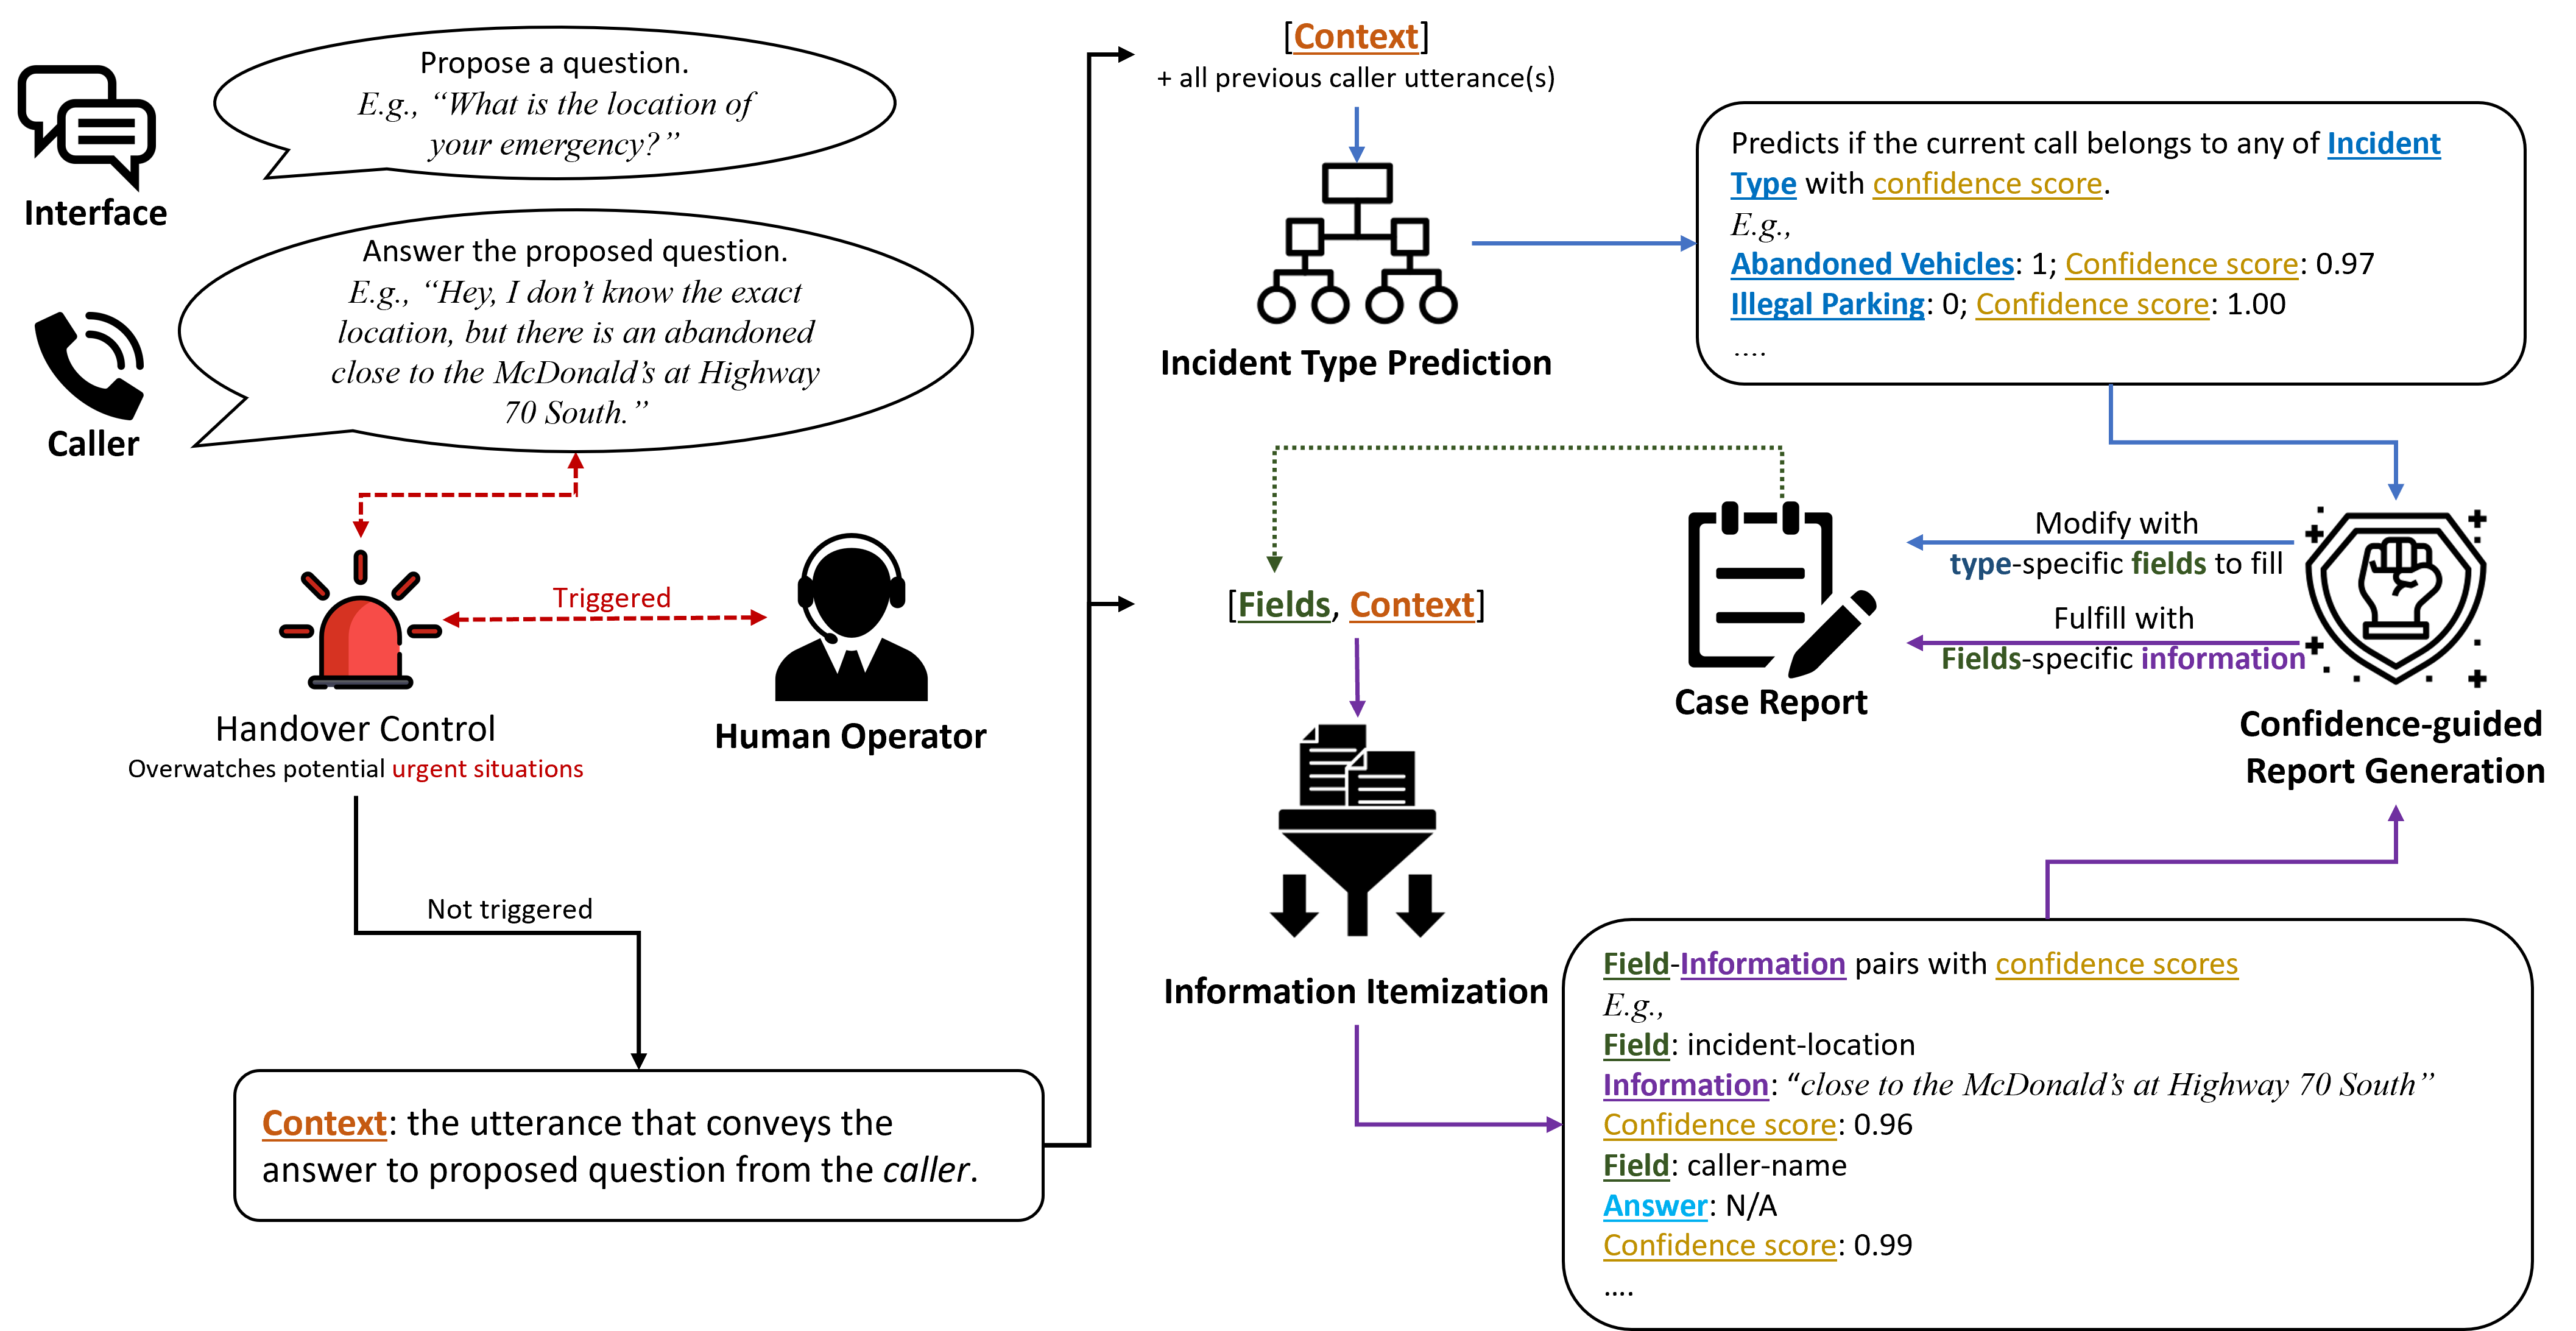
\includegraphics[width=0.9\textwidth]{figures/running_example.png}
    \caption{Running Example within One Turn of Conversation}
    \label{fig:running_example}
    \vspace{-0.5cm}
\end{figure*}

Our dataset includes real-world audio recordings covering from November 2022 to February 2023 across over 11 non-emergency types, we focus on the most common 11 incident types in this paper. Incident types are carefully annotated by dispatchers from the emergency response center.

In this section, we introduce our dataset in more detail. Initially, the dataset consists of 11,796 real recordings from the local call center. To convert the audio files in textual format for Auto311 to learn, we transcribe the audio with speaker diarization \cite{openai_whisper_2022, Bredin_pyannote_2020}. Following is one sample transcription from our dataset reporting an abandoned vehicle with private and sensitive information masked.

\noindent[00:00:13.727]--[00:00:16.458] $\mathsf{Dispatcher}$: Police Fire and Medical. 

\noindent[00:00:17.121]--[00:00:36.458] $\mathsf{Caller}$: Oh, good morning. Um, there is a car that seems to be abandoned, uh, across the street. And I just wondered if someone could check it out. It hasn't moved in weeks and weeks and weeks, and it's got kind of tinted windows and it's just creepy.

\noindent[00:00:36.863]--[00:00:38.061] $\mathsf{Dispatcher}$:  Okay, where is it located?

\noindent[00:00:39.023]--[00:01:05.483] $\mathsf{Caller}$: It is across the street from \textit{\#masked\_address}, and that's \textit{\#masked\_address}. It's in front of like a very small green space. There are kids that play in that green space, and we just all kind of, you know, creeped out about it.

\noindent[00:01:05.685]--[00:01:11.372] $\mathsf{Dispatcher}$:  Okay, so \textit{\#masked\_address}. What kind of vehicle is it?

\noindent[00:01:12.182]--[00:01:31.842] $\mathsf{Caller}$:  It is a very dark grey Volvo I believe is what it is. It's a very dark grey car and the windows are tinted just a bit.

\noindent[00:01:35.740]--[00:01:47.316] $\mathsf{Dispatcher}$: Alright, and what's your first and last name?

\noindent[00:01:48.261]--[00:01:49.746] $\mathsf{Caller}$: Okay, my name is \textit{\#masked\_personal\_information}.

\noindent[00:01:50.421]--[00:01:52.598] $\mathsf{Dispatcher}$: Did you want to speak to an officer when they come out?

\noindent[00:01:53.340]--[00:01:55.517] $\mathsf{Caller}$:  No, there's no need for that.

\noindent[00:01:55.956]--[00:02:05.204] $\mathsf{Dispatcher}$:  Alright, I will get someone out there across \textit{\#masked\_address} as soon as we can, okay?

\noindent[00:02:05.912]--[00:02:09.642] $\mathsf{Caller}$:  That sounds great. Thank you so much and I hope you have a real good day.

\noindent[00:02:09.574]--[00:02:10.013] $\mathsf{Dispatcher}$:  You too, bye.



\section{One Example Turn of Auto311}
A further example in Auto311 is also provided in Figure \ref{fig:running_example}.

\section{Handover Control Patterns}

We denote the ongoing user utterance as $\mathsf{S}$, the set of patterns as $p_0, p_1, ..., p_n \subset \mathsf{P}$, and the whole process as a boolean function $\mathsf{is\_trigger(S, {P})}$. Our rule-based procedure can be concluded using the following pseudo-logic: 

``if any pattern $p$ of $\mathsf{P}$ exists in $\mathsf{S}$, then $\mathsf{is\_trigger(S, {P})}$ returns true, the handover control is triggered, and the system interactions will be ceased and the call will be rerouted to a real operator immediately. Otherwise, $\mathsf{is\_trigger(S, {P})}$ returns false and the handover control continues over-watching the ongoing call.'' 

\begin{table}[h]
\centering
\scriptsize
\caption{Example patterns in handover control}
\begin{tabular}{||c|c|c||}
\hline
Cases                                       & Example Patterns             & Example Texts      \\ \hline\hline
\multirow{2}{*}{Request Human Operators} & {[}NP$\ast${]}                    & real human         \\ \cline{2-3} 
                                            & {[}VP$\ast${]}                    & end the call       \\ \hline
\multirow{2}{*}{Alert Potential Urgency} & {[}PRP{]}{[}be{]}{[}ADJP$\ast${]} & he is unresponsive \\ \cline{2-3} 
                                            & {[}VP$\ast${]}{[}be{]}{[}NP$\ast${]}   & guns are fired     \\ \hline
\end{tabular}
\label{tab:patterns}
\end{table}

Here we provide several patterns in Table \ref{tab:patterns}, where VP, NP, PRP, ADJP, and PP refer to verb phrases, noun phrases, personal phrases, adjective phrases, and prepositional phrases. We mark phrases that need to be maintained during runtime using sensitive keywords using stars ($\ast$). Note, this is not an exhaustive table, both patterns and sensitive keywords will be extended during usage.




\section{Phone tree of Incident Types}
We work with city authorities and create the following phone tree for different incident types, including 11 types of incidents including, illegal parking, abandoned vehicle, aggressive driver, lost-stolen, damaged property, found property, drug pros, check welfare, and noise violation. Each event has its only specific fields to fill alongside each call. The phone tree is in Figure \ref{fig:phone_tree}, we only show 9 incident types here due to the page size.


\subsection{Additional Evaluation} 

\begin{table}[]
\footnotesize
\begin{tabular}{||c|cccc||}
\hline
          & \multicolumn{4}{c||}{Illegal Parking(binary)}                                                                                                 \\ \hline\hline
Metric    & \multicolumn{1}{c|}{Precision}         & \multicolumn{1}{c|}{Recall}            & \multicolumn{1}{c|}{F-1}               & Accuracy          \\ \hline
LSTM      & \multicolumn{1}{c|}{53.85\%}           & \multicolumn{1}{c|}{87.79\%}           & \multicolumn{1}{c|}{70.00\%}           & 53.85\%           \\ \hline
CNN       & \multicolumn{1}{c|}{0.00\%}                 & \multicolumn{1}{c|}{0.00\%}                 & \multicolumn{1}{c|}{0.00\%}                 & 0.00\%                 \\ \hline
RCNN      & \multicolumn{1}{c|}{0.00\%}                 & \multicolumn{1}{c|}{0.00\%}                 & \multicolumn{1}{c|}{0.00\%}                 & 0.00\%                 \\ \hline
RNN       & \multicolumn{1}{c|}{25.00\%}           & \multicolumn{1}{c|}{28.57\%}           & \multicolumn{1}{c|}{26.67\%}           & 15.38\%           \\ \hline
Self-Attn & \multicolumn{1}{c|}{0.00\%}                 & \multicolumn{1}{c|}{0.00\%}                 & \multicolumn{1}{c|}{0.00\%}                 & 0.00\%                 \\ \hline
Attention & \multicolumn{1}{c|}{55.56\%}           & \multicolumn{1}{c|}{71.42\%}           & \multicolumn{1}{c|}{62.50\%}           & 53.85\%           \\ \hline
Bert      & \multicolumn{1}{c|}{100.00\%} & \multicolumn{1}{c|}{100.00\%} & \multicolumn{1}{c|}{100.00\%} & 100.00\% \\ \hline
\textbf{Auto311}   & \multicolumn{1}{c|}{\textbf{100.00\%}} & \multicolumn{1}{c|}{\textbf{100.00\%}} & \multicolumn{1}{c|}{\textbf{100.00\%}} & \textbf{100.00\%} \\ \hline
\end{tabular}
\label{table:rest_eval}
\caption{Auto311 on Incident Type Prediction}
\end{table}

\subsubsection{Evaluation on Incident Type Prediction}
Here we provide the rest evaluation of Auto311 on incident prediction, specifically on illegal parking and found property. The last layer of the incident type prediction module contains a binary classification of illegal parking and found property, see Table 4 for more details. As we can tell from the table, with the introduction of confidence guidance, Auto311 leverages the strong prior knowledge from BERT, yielding 100.00\% F-1 scores on both incident types.


% \section{Phone Tree to Handle Different Incident Type}



\subsubsection{Validating Proposed Metric for Text Comparison}

We conduct an evaluation to assess the effectiveness of our proposed text comparison metric, targeting the question ``How does this new text comparison work in this specific scenario?''. For this evaluation, we manually selected three distinct groups of text pairs:
\begin{itemize}
    \item \textbf{Group one} consists of text pairs that are entirely dissimilar, for instance, ``65 South exit 92'' and ``Silver Camaro.'' These pairs serve as a benchmark to evaluate how well the metric can discern vastly different information.
    \item \textbf{Group two} comprises pairs that exhibit slight differences in their content, but these discrepancies are not significant enough to significantly impact the dispatcher's decision-making process. For example, pairs like ``an SUV type truck'' and ``It's like an SUV type truck, maybe a Tahoe'' fall under this category.
    \item \textbf{Group three} contains pairs with identical or highly similar information, which are relevant for dispatchers to complete internal reports. Examples of such pairs include ``on the West End Ave'' and ``West End Ave.''
\end{itemize}

To test the consistency scores, we utilize traditional metrics like BLEU \cite{papineni2002bleu}, Damerau–Levenshtein Distance (DLD) \cite{damerau1964technique}, and ROUGE \cite{lin-2004-rouge}, in addition to our modified metric. The evaluation aims to compare how each metric performs in distinguishing differences and similarities within the text pairs across these distinct groups. This analysis will provide valuable insights into the efficacy of our proposed metric compared to established text comparison metrics.

\begin{figure}[h]
    \centering
    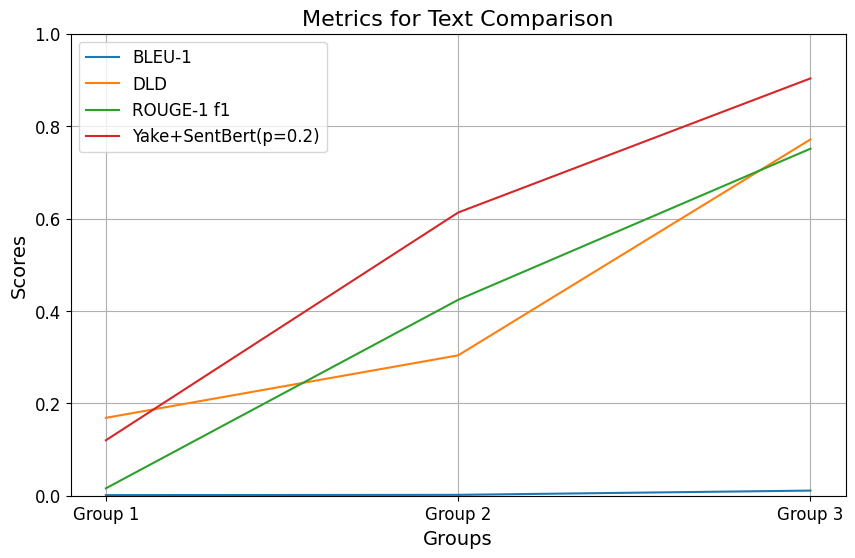
\includegraphics[width=0.40\textwidth]{figures/line-graph.png}
    \caption{Metric for Text Comparison}
    \label{fig:textcompare}
    \vspace{-0.5cm}
\end{figure}

Analysis of the plot reveals certain transitional metrics display an upward trend while failing to furnish a fair assessment. The ideal metric yields low scores for group one pair comparisons and high scores for group three pairs. As Figure \ref{fig:textcompare} displays, although exhibiting increased scores from group one to group three, DLD and ROUGE do not account for the robust correlations among text pairs in group three.

% From analyzing the plot, it is clear that some of the transitional metrics exhibit an upward trend, yet they do not provide a just assessment score. Ideally, we require a metric that yields a low score when comparing group one pairs and a high score when comparing group three pairs. The plot displays in figure \ref{fig:textcompare} reveals that DLD and ROUGE, despite their increasing scores from group 1 to group 3, fail to account for the high correlations among text pairs in group 3. 

\textit{Ultimately, from the results, it indicates our proposed text comparison metric proves more effective in assessing texts for consistency in this non-emergency dispatching scenario.}

% The objective is to demonstrate the effectiveness of the text comparison method we propose. We ask dispatchers to (1) evaluate the consistency among a list of texts in a real-world dispatching task, (2) compare our metric with their score, and (3) ask them if the scores make more sense.



\section{Discussion and Future Work}
This section discusses potential future work to enhance our proposed system based on additional findings from dataset review and development planning.

\subsubsection{Address Validation}
Location information is critical in emergency response systems. However, callers often describe locations using landmarks, not addresses. Descriptions like ``the McDonald's at Charlotte Pike'' are implicit. Translating these to explicit addresses or coordinates could better locate incidents. This work highlights address information from caller utterances without additional validation.

% Location information remains critical in an emergency and non-emergency response systems. However, callers frequently describe locations using conspicuous buildings or common spots during phone conversations. These qualitative location descriptions warrant further validation or clarification for location-sensitive tasks like emergency response. For instance, locations such as ``the McDonald's at Charlotte Pike'' or ``the Walmart entrance'' constitute implicit or ambiguous information. Hence, translating casual descriptions into explicit address details, ideally, coordinates, could better locate incidents. Presently, this work solely highlights address information from caller utterances without additional validation.

\subsubsection{Redundant Call and Callback Handling}
Redundant calls frequently occur reporting identical incidents. For instance, when witnesses spot a highway car crash, multiple people may call to report the same event, providing descriptions like ``there is a car wreck on I-440, milestone 76'' or ``there is a severe car crash on Interstate 440.'' While calling about the same incident, each call can still furnish unique unobtainable information. Similarly, caller callbacks regarding the same incident often provide previously omitted details, e.g., ``Hey, I just called a few minutes ago reporting an aggressive driver on I-40, I think the driver is in a blue Toyota, I just saw him.'' Hence, skipping or terminating ostensibly redundant calls proves inappropriate. Instead, solutions should strategically emphasize novel information despite referring to a previously reported incident. Presently, we treat each incoming call equivalently without assigning differential importance to any information we attempt to collect.


\begin{figure*}[ht]
\centering
\rotatebox{90}{
  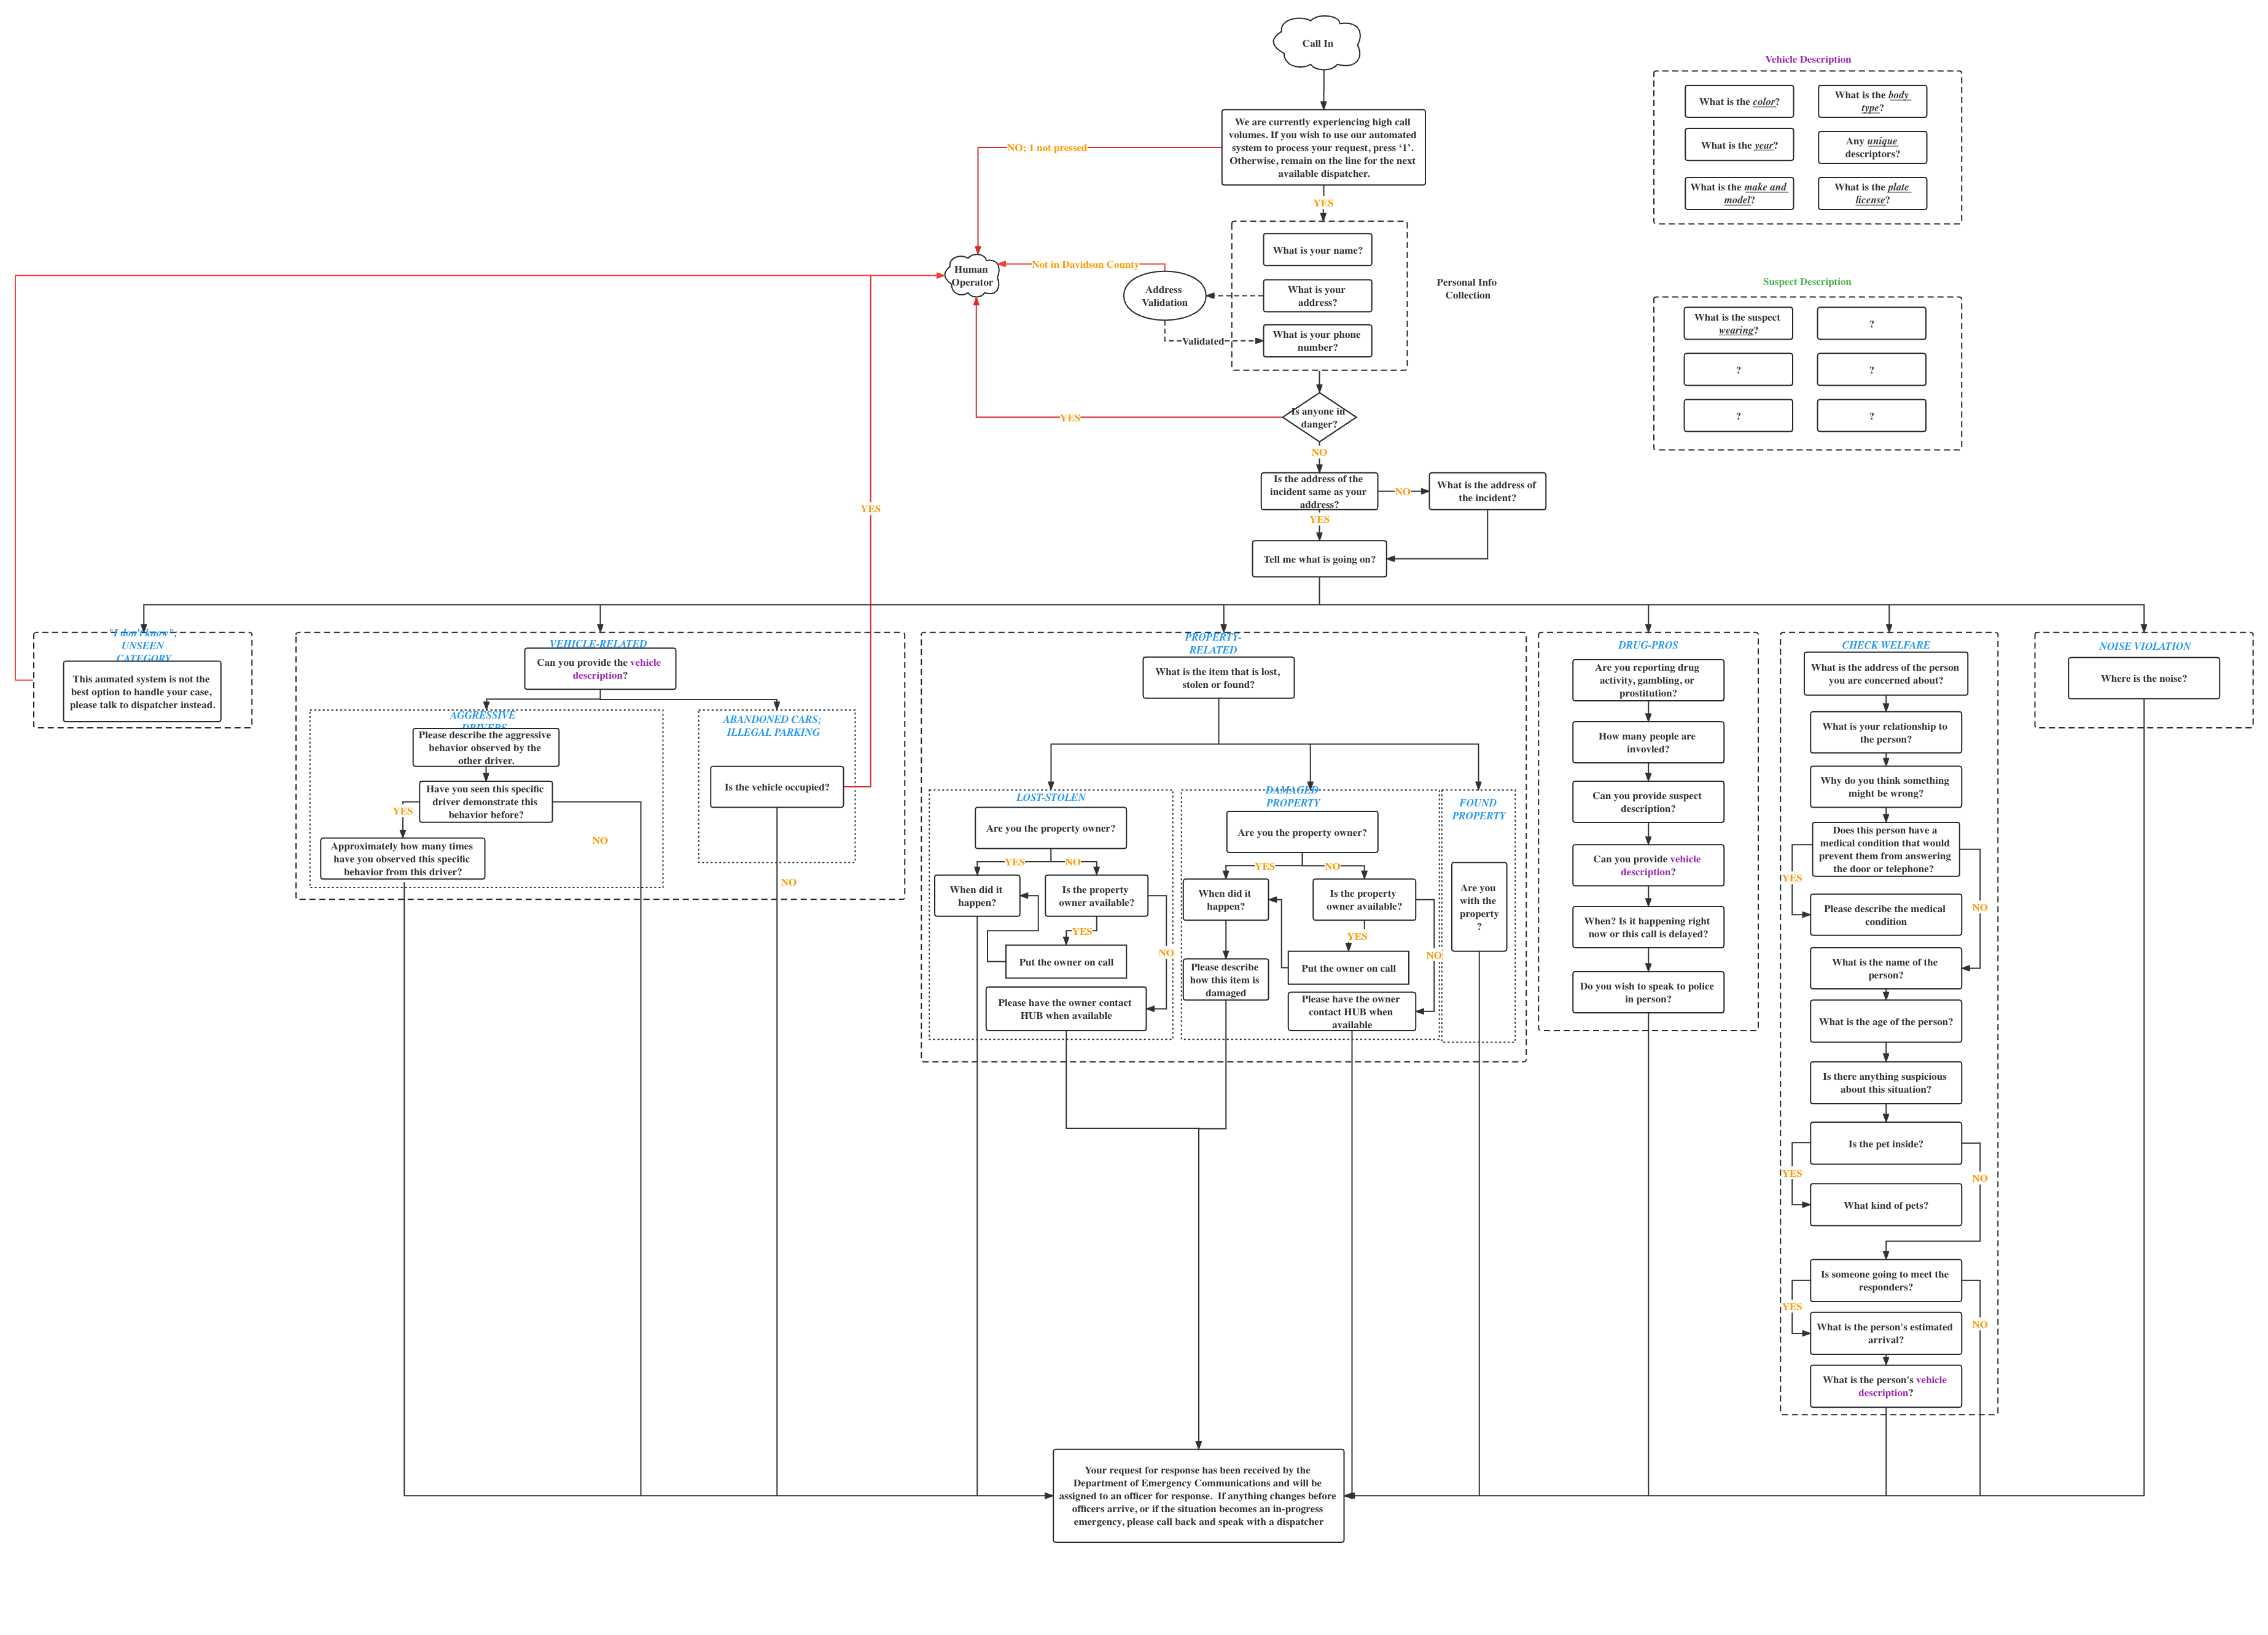
\includegraphics[width=1.4\textwidth]{figures/CIVIC-311.png} 
}
\caption{Phone Tree for Incident Handling} 
\label{fig:phone_tree}
\end{figure*}

\begin{table}[]
\footnotesize
\begin{tabular}{||c|c|c|c|c||}
\hline
          & Minor Crash Report & Lost-Stolen & Aggressive Drivers & Damaged Property \\ \hline\hline
LSTM      & 56.47\%            & 0.00\%      & 53.85\%            & 0.00\%           \\ \hline
CNN       & 75.86\%            & 85.71\%     & 72.72\%            & 40.00\%          \\ \hline
RCNN      & 90.57\%            & 82.35\%     & 61.54\%            & 76.92\%          \\ \hline
RNN       & 63.33\%            & 40.00\%     & 52.71\%            & 44.44\%          \\ \hline
Self-Attn & 88.46\%            & 88.89\%     & 66.67\%            & 66.67\%          \\ \hline
Attention & 91.69\%            & 62.50\%     & 50.00\%            & 54.55\%          \\ \hline
Bert      & 95.04\%            & 95.60\%     & 92.31\%            & 88.89\%          \\ \hline
\textbf{Auto311}   & \textbf{95.71\%}            & \textbf{96.70\%}     & \textbf{93.75\%}            & \textbf{94.12\%}          \\ \hline
\end{tabular}
\end{table}